% Options for packages loaded elsewhere
\PassOptionsToPackage{unicode}{hyperref}
\PassOptionsToPackage{hyphens}{url}
%
\documentclass[
  doc]{apa6}
\usepackage{amsmath,amssymb}
\usepackage{iftex}
\ifPDFTeX
  \usepackage[T1]{fontenc}
  \usepackage[utf8]{inputenc}
  \usepackage{textcomp} % provide euro and other symbols
\else % if luatex or xetex
  \usepackage{unicode-math} % this also loads fontspec
  \defaultfontfeatures{Scale=MatchLowercase}
  \defaultfontfeatures[\rmfamily]{Ligatures=TeX,Scale=1}
\fi
\usepackage{lmodern}
\ifPDFTeX\else
  % xetex/luatex font selection
\fi
% Use upquote if available, for straight quotes in verbatim environments
\IfFileExists{upquote.sty}{\usepackage{upquote}}{}
\IfFileExists{microtype.sty}{% use microtype if available
  \usepackage[]{microtype}
  \UseMicrotypeSet[protrusion]{basicmath} % disable protrusion for tt fonts
}{}
\makeatletter
\@ifundefined{KOMAClassName}{% if non-KOMA class
  \IfFileExists{parskip.sty}{%
    \usepackage{parskip}
  }{% else
    \setlength{\parindent}{0pt}
    \setlength{\parskip}{6pt plus 2pt minus 1pt}}
}{% if KOMA class
  \KOMAoptions{parskip=half}}
\makeatother
\usepackage{xcolor}
\usepackage{color}
\usepackage{fancyvrb}
\newcommand{\VerbBar}{|}
\newcommand{\VERB}{\Verb[commandchars=\\\{\}]}
\DefineVerbatimEnvironment{Highlighting}{Verbatim}{commandchars=\\\{\}}
% Add ',fontsize=\small' for more characters per line
\usepackage{framed}
\definecolor{shadecolor}{RGB}{248,248,248}
\newenvironment{Shaded}{\begin{snugshade}}{\end{snugshade}}
\newcommand{\AlertTok}[1]{\textcolor[rgb]{0.94,0.16,0.16}{#1}}
\newcommand{\AnnotationTok}[1]{\textcolor[rgb]{0.56,0.35,0.01}{\textbf{\textit{#1}}}}
\newcommand{\AttributeTok}[1]{\textcolor[rgb]{0.13,0.29,0.53}{#1}}
\newcommand{\BaseNTok}[1]{\textcolor[rgb]{0.00,0.00,0.81}{#1}}
\newcommand{\BuiltInTok}[1]{#1}
\newcommand{\CharTok}[1]{\textcolor[rgb]{0.31,0.60,0.02}{#1}}
\newcommand{\CommentTok}[1]{\textcolor[rgb]{0.56,0.35,0.01}{\textit{#1}}}
\newcommand{\CommentVarTok}[1]{\textcolor[rgb]{0.56,0.35,0.01}{\textbf{\textit{#1}}}}
\newcommand{\ConstantTok}[1]{\textcolor[rgb]{0.56,0.35,0.01}{#1}}
\newcommand{\ControlFlowTok}[1]{\textcolor[rgb]{0.13,0.29,0.53}{\textbf{#1}}}
\newcommand{\DataTypeTok}[1]{\textcolor[rgb]{0.13,0.29,0.53}{#1}}
\newcommand{\DecValTok}[1]{\textcolor[rgb]{0.00,0.00,0.81}{#1}}
\newcommand{\DocumentationTok}[1]{\textcolor[rgb]{0.56,0.35,0.01}{\textbf{\textit{#1}}}}
\newcommand{\ErrorTok}[1]{\textcolor[rgb]{0.64,0.00,0.00}{\textbf{#1}}}
\newcommand{\ExtensionTok}[1]{#1}
\newcommand{\FloatTok}[1]{\textcolor[rgb]{0.00,0.00,0.81}{#1}}
\newcommand{\FunctionTok}[1]{\textcolor[rgb]{0.13,0.29,0.53}{\textbf{#1}}}
\newcommand{\ImportTok}[1]{#1}
\newcommand{\InformationTok}[1]{\textcolor[rgb]{0.56,0.35,0.01}{\textbf{\textit{#1}}}}
\newcommand{\KeywordTok}[1]{\textcolor[rgb]{0.13,0.29,0.53}{\textbf{#1}}}
\newcommand{\NormalTok}[1]{#1}
\newcommand{\OperatorTok}[1]{\textcolor[rgb]{0.81,0.36,0.00}{\textbf{#1}}}
\newcommand{\OtherTok}[1]{\textcolor[rgb]{0.56,0.35,0.01}{#1}}
\newcommand{\PreprocessorTok}[1]{\textcolor[rgb]{0.56,0.35,0.01}{\textit{#1}}}
\newcommand{\RegionMarkerTok}[1]{#1}
\newcommand{\SpecialCharTok}[1]{\textcolor[rgb]{0.81,0.36,0.00}{\textbf{#1}}}
\newcommand{\SpecialStringTok}[1]{\textcolor[rgb]{0.31,0.60,0.02}{#1}}
\newcommand{\StringTok}[1]{\textcolor[rgb]{0.31,0.60,0.02}{#1}}
\newcommand{\VariableTok}[1]{\textcolor[rgb]{0.00,0.00,0.00}{#1}}
\newcommand{\VerbatimStringTok}[1]{\textcolor[rgb]{0.31,0.60,0.02}{#1}}
\newcommand{\WarningTok}[1]{\textcolor[rgb]{0.56,0.35,0.01}{\textbf{\textit{#1}}}}
\usepackage{graphicx}
\makeatletter
\def\maxwidth{\ifdim\Gin@nat@width>\linewidth\linewidth\else\Gin@nat@width\fi}
\def\maxheight{\ifdim\Gin@nat@height>\textheight\textheight\else\Gin@nat@height\fi}
\makeatother
% Scale images if necessary, so that they will not overflow the page
% margins by default, and it is still possible to overwrite the defaults
% using explicit options in \includegraphics[width, height, ...]{}
\setkeys{Gin}{width=\maxwidth,height=\maxheight,keepaspectratio}
% Set default figure placement to htbp
\makeatletter
\def\fps@figure{htbp}
\makeatother
\setlength{\emergencystretch}{3em} % prevent overfull lines
\providecommand{\tightlist}{%
  \setlength{\itemsep}{0pt}\setlength{\parskip}{0pt}}
\setcounter{secnumdepth}{5}
% Make \paragraph and \subparagraph free-standing
\ifx\paragraph\undefined\else
  \let\oldparagraph\paragraph
  \renewcommand{\paragraph}[1]{\oldparagraph{#1}\mbox{}}
\fi
\ifx\subparagraph\undefined\else
  \let\oldsubparagraph\subparagraph
  \renewcommand{\subparagraph}[1]{\oldsubparagraph{#1}\mbox{}}
\fi
\newlength{\cslhangindent}
\setlength{\cslhangindent}{1.5em}
\newlength{\csllabelwidth}
\setlength{\csllabelwidth}{3em}
\newlength{\cslentryspacingunit} % times entry-spacing
\setlength{\cslentryspacingunit}{\parskip}
\newenvironment{CSLReferences}[2] % #1 hanging-ident, #2 entry spacing
 {% don't indent paragraphs
  \setlength{\parindent}{0pt}
  % turn on hanging indent if param 1 is 1
  \ifodd #1
  \let\oldpar\par
  \def\par{\hangindent=\cslhangindent\oldpar}
  \fi
  % set entry spacing
  \setlength{\parskip}{#2\cslentryspacingunit}
 }%
 {}
\usepackage{calc}
\newcommand{\CSLBlock}[1]{#1\hfill\break}
\newcommand{\CSLLeftMargin}[1]{\parbox[t]{\csllabelwidth}{#1}}
\newcommand{\CSLRightInline}[1]{\parbox[t]{\linewidth - \csllabelwidth}{#1}\break}
\newcommand{\CSLIndent}[1]{\hspace{\cslhangindent}#1}
\ifLuaTeX
\usepackage[bidi=basic]{babel}
\else
\usepackage[bidi=default]{babel}
\fi
\babelprovide[main,import]{english}
% get rid of language-specific shorthands (see #6817):
\let\LanguageShortHands\languageshorthands
\def\languageshorthands#1{}
% Manuscript styling
\usepackage{upgreek}
\captionsetup{font=singlespacing,justification=justified}

% Table formatting
\usepackage{longtable}
\usepackage{lscape}
% \usepackage[counterclockwise]{rotating}   % Landscape page setup for large tables
\usepackage{multirow}		% Table styling
\usepackage{tabularx}		% Control Column width
\usepackage[flushleft]{threeparttable}	% Allows for three part tables with a specified notes section
\usepackage{threeparttablex}            % Lets threeparttable work with longtable

% Create new environments so endfloat can handle them
% \newenvironment{ltable}
%   {\begin{landscape}\centering\begin{threeparttable}}
%   {\end{threeparttable}\end{landscape}}
\newenvironment{lltable}{\begin{landscape}\centering\begin{ThreePartTable}}{\end{ThreePartTable}\end{landscape}}

% Enables adjusting longtable caption width to table width
% Solution found at http://golatex.de/longtable-mit-caption-so-breit-wie-die-tabelle-t15767.html
\makeatletter
\newcommand\LastLTentrywidth{1em}
\newlength\longtablewidth
\setlength{\longtablewidth}{1in}
\newcommand{\getlongtablewidth}{\begingroup \ifcsname LT@\roman{LT@tables}\endcsname \global\longtablewidth=0pt \renewcommand{\LT@entry}[2]{\global\advance\longtablewidth by ##2\relax\gdef\LastLTentrywidth{##2}}\@nameuse{LT@\roman{LT@tables}} \fi \endgroup}

% \setlength{\parindent}{0.5in}
% \setlength{\parskip}{0pt plus 0pt minus 0pt}

% Overwrite redefinition of paragraph and subparagraph by the default LaTeX template
% See https://github.com/crsh/papaja/issues/292
\makeatletter
\renewcommand{\paragraph}{\@startsection{paragraph}{4}{\parindent}%
  {0\baselineskip \@plus 0.2ex \@minus 0.2ex}%
  {-1em}%
  {\normalfont\normalsize\bfseries\itshape\typesectitle}}

\renewcommand{\subparagraph}[1]{\@startsection{subparagraph}{5}{1em}%
  {0\baselineskip \@plus 0.2ex \@minus 0.2ex}%
  {-\z@\relax}%
  {\normalfont\normalsize\itshape\hspace{\parindent}{#1}\textit{\addperi}}{\relax}}
\makeatother

\makeatletter
\usepackage{etoolbox}
\patchcmd{\maketitle}
  {\section{\normalfont\normalsize\abstractname}}
  {\section*{\normalfont\normalsize\abstractname}}
  {}{\typeout{Failed to patch abstract.}}
\patchcmd{\maketitle}
  {\section{\protect\normalfont{\@title}}}
  {\section*{\protect\normalfont{\@title}}}
  {}{\typeout{Failed to patch title.}}
\makeatother

\usepackage{xpatch}
\makeatletter
\xapptocmd\appendix
  {\xapptocmd\section
    {\addcontentsline{toc}{section}{\appendixname\ifoneappendix\else~\theappendix\fi\\: #1}}
    {}{\InnerPatchFailed}%
  }
{}{\PatchFailed}
\usepackage{csquotes}
\ifLuaTeX
  \usepackage{selnolig}  % disable illegal ligatures
\fi
\IfFileExists{bookmark.sty}{\usepackage{bookmark}}{\usepackage{hyperref}}
\IfFileExists{xurl.sty}{\usepackage{xurl}}{} % add URL line breaks if available
\urlstyle{same}
\hypersetup{
  pdftitle={Weighting, data management and regression},
  pdfauthor={Prof.~Dr.~Stephan Huber1,2},
  pdflang={en-EN},
  hidelinks,
  pdfcreator={LaTeX via pandoc}}

\title{Weighting, data management and regression}
\author{Prof.~Dr.~Stephan Huber\textsuperscript{1,2}}
\date{}


\shorttitle{Weighting, data management and regression}

\authornote{

All files related to this document can be found here: \url{https://github.com/hubchev/ewa}. Please contact us via \texttt{stephan.huber@hs-fresenius.de}.

}

\affiliation{\vspace{0.5cm}\textsuperscript{1} Fresenius University of Applied Science\\\textsuperscript{2} Charlotte Fresenius University}

\abstract{%
In this document I show what weighted means and their distribution are all about. Furthermore, I show some possibilities of data management in R with the \texttt{dplyr} package and how a regression analysis in R is performed and visualised.
}



\begin{document}
\maketitle

\newpage

\hypertarget{solutions-and-cheatsheet}{%
\section{Solutions and Cheatsheet}\label{solutions-and-cheatsheet}}

Please consider the report you find here:

\url{https://hubchev.github.io/various/exam_functions.html}

In this report, I summarize operators and popular functions of R. Moreover, I present the output of all exercises. That should help you to write code and start to look for solutions to your challenges in working with data:

\hypertarget{datenmanagement}{%
\section{Datenmanagement}\label{datenmanagement}}

\begin{table}

\caption{\label{tab:data1}Data}
\centering
\begin{tabular}[t]{l|l|r|l}
\hline
v1 & v2 & v3 & v4\\
\hline
1 & A & NA & \\
\hline
2 & NA & 0.2 & 0.4\\
\hline
 & C & 0.3 & 0.1\\
\hline
4 & D & NA & 3\\
\hline
5 & E & 0.5 & 1.5\\
\hline
\end{tabular}
\end{table}

Consider the data of Table \ref{tab:data1} and solve the following exercises:

\begin{enumerate}
\def\labelenumi{\alph{enumi})}
\tightlist
\item
  Add variable \texttt{misone} that is 1 if there is a missing and 0 otherwise.
  \emph{(Hint: Use \texttt{case\_when} and \texttt{is.na()}.)}
\end{enumerate}

\newpage

\begin{Shaded}
\begin{Highlighting}[]
\NormalTok{df }\OtherTok{\textless{}{-}}\NormalTok{ df }\SpecialCharTok{|\textgreater{}} 
  \FunctionTok{mutate}\NormalTok{(}\AttributeTok{misone =} \FunctionTok{case\_when}\NormalTok{(}
\NormalTok{    v1 }\SpecialCharTok{==} \StringTok{""} \SpecialCharTok{|} \FunctionTok{is.na}\NormalTok{(v1) }\SpecialCharTok{\textasciitilde{}} \DecValTok{1}\NormalTok{,}
\NormalTok{    v2 }\SpecialCharTok{==} \StringTok{""} \SpecialCharTok{|} \FunctionTok{is.na}\NormalTok{(v2) }\SpecialCharTok{\textasciitilde{}} \DecValTok{1}\NormalTok{,}
\NormalTok{    v3 }\SpecialCharTok{==} \StringTok{""} \SpecialCharTok{|} \FunctionTok{is.na}\NormalTok{(v3) }\SpecialCharTok{\textasciitilde{}} \DecValTok{1}\NormalTok{,}
\NormalTok{    v4 }\SpecialCharTok{==} \StringTok{""} \SpecialCharTok{|} \FunctionTok{is.na}\NormalTok{(v4) }\SpecialCharTok{\textasciitilde{}} \DecValTok{1}\NormalTok{,}
    \ConstantTok{TRUE} \SpecialCharTok{\textasciitilde{}} \DecValTok{0} 
\NormalTok{  ))}

\NormalTok{knitr}\SpecialCharTok{::}\FunctionTok{kable}\NormalTok{(df, }\StringTok{"latex"}\NormalTok{, }\AttributeTok{caption =} \StringTok{"Solution a)"}\NormalTok{)}
\end{Highlighting}
\end{Shaded}

\begin{table}

\caption{\label{tab:unnamed-chunk-2}Solution a)}
\centering
\begin{tabular}[t]{l|l|r|l|r}
\hline
v1 & v2 & v3 & v4 & misone\\
\hline
1 & A & NA &  & 1\\
\hline
2 & NA & 0.2 & 0.4 & 1\\
\hline
 & C & 0.3 & 0.1 & 1\\
\hline
4 & D & NA & 3 & 1\\
\hline
5 & E & 0.5 & 1.5 & 0\\
\hline
\end{tabular}
\end{table}

\newpage

\begin{enumerate}
\def\labelenumi{\alph{enumi})}
\setcounter{enumi}{1}
\tightlist
\item
  Add variable \texttt{miscount} that counts how many observations are missing in each row.
  \emph{(Hint: Use \texttt{mutate\_all}, \texttt{rowSums}, and \texttt{pick(everything())})}
\end{enumerate}

\newpage

\begin{Shaded}
\begin{Highlighting}[]
\NormalTok{test\_df }\OtherTok{\textless{}{-}}\NormalTok{ df }\SpecialCharTok{|\textgreater{}} 
  \FunctionTok{mutate\_all}\NormalTok{(}\SpecialCharTok{\textasciitilde{}} \FunctionTok{if\_else}\NormalTok{(}\FunctionTok{is.na}\NormalTok{(.) }\SpecialCharTok{|}\NormalTok{ . }\SpecialCharTok{==} \StringTok{""}\NormalTok{, }\DecValTok{1}\NormalTok{, }\DecValTok{0}\NormalTok{)) }\SpecialCharTok{|\textgreater{}}
  \FunctionTok{mutate}\NormalTok{(}\AttributeTok{miscount =} \FunctionTok{rowSums}\NormalTok{(}\FunctionTok{pick}\NormalTok{(}\FunctionTok{everything}\NormalTok{())))}

\NormalTok{test\_df\_miscount }\OtherTok{\textless{}{-}}\NormalTok{ test\_df }\SpecialCharTok{|\textgreater{}} 
  \FunctionTok{select}\NormalTok{(miscount) }
  
\NormalTok{df }\OtherTok{\textless{}{-}} \FunctionTok{bind\_cols}\NormalTok{(df, test\_df\_miscount)}

\NormalTok{knitr}\SpecialCharTok{::}\FunctionTok{kable}\NormalTok{(df, }\StringTok{"latex"}\NormalTok{, }\AttributeTok{caption =} \StringTok{"Solution b)"}\NormalTok{)}
\end{Highlighting}
\end{Shaded}

\begin{table}

\caption{\label{tab:unnamed-chunk-3}Solution b)}
\centering
\begin{tabular}[t]{l|l|r|l|r|r}
\hline
v1 & v2 & v3 & v4 & misone & miscount\\
\hline
1 & A & NA &  & 1 & 2\\
\hline
2 & NA & 0.2 & 0.4 & 1 & 1\\
\hline
 & C & 0.3 & 0.1 & 1 & 1\\
\hline
4 & D & NA & 3 & 1 & 1\\
\hline
5 & E & 0.5 & 1.5 & 0 & 0\\
\hline
\end{tabular}
\end{table}

\newpage

\begin{enumerate}
\def\labelenumi{\alph{enumi})}
\setcounter{enumi}{2}
\tightlist
\item
  Use the function \texttt{rowwise} to calculate the \texttt{NA} and \texttt{""} observations.
  \emph{(Hint: Use \texttt{is.na} and \texttt{pick(everything())}.)}
\end{enumerate}

\newpage

\begin{Shaded}
\begin{Highlighting}[]
\NormalTok{df }\OtherTok{\textless{}{-}}\NormalTok{ df }\SpecialCharTok{|\textgreater{}} 
  \FunctionTok{rowwise}\NormalTok{() }\SpecialCharTok{|\textgreater{}} 
  \FunctionTok{mutate}\NormalTok{(}\AttributeTok{count\_NA =} \FunctionTok{sum}\NormalTok{(}\FunctionTok{is.na}\NormalTok{(}\FunctionTok{pick}\NormalTok{(}\FunctionTok{everything}\NormalTok{())))) }\SpecialCharTok{|\textgreater{}} 
  \FunctionTok{mutate}\NormalTok{(}\AttributeTok{count\_OK =} \FunctionTok{sum}\NormalTok{(}\FunctionTok{pick}\NormalTok{(}\FunctionTok{everything}\NormalTok{()) }\SpecialCharTok{==} \StringTok{""}\NormalTok{, }\AttributeTok{na.rm =} \ConstantTok{TRUE}\NormalTok{)) }\SpecialCharTok{|\textgreater{}} 
  \FunctionTok{ungroup}\NormalTok{()}

\NormalTok{knitr}\SpecialCharTok{::}\FunctionTok{kable}\NormalTok{(df, }\StringTok{"latex"}\NormalTok{, }\AttributeTok{caption =} \StringTok{"Solution c)"}\NormalTok{)}
\end{Highlighting}
\end{Shaded}

\begin{table}

\caption{\label{tab:unnamed-chunk-4}Solution c)}
\centering
\begin{tabular}[t]{l|l|r|l|r|r|r|r}
\hline
v1 & v2 & v3 & v4 & misone & miscount & count\_NA & count\_OK\\
\hline
1 & A & NA &  & 1 & 2 & 1 & 1\\
\hline
2 & NA & 0.2 & 0.4 & 1 & 1 & 1 & 0\\
\hline
 & C & 0.3 & 0.1 & 1 & 1 & 0 & 1\\
\hline
4 & D & NA & 3 & 1 & 1 & 1 & 0\\
\hline
5 & E & 0.5 & 1.5 & 0 & 0 & 0 & 0\\
\hline
\end{tabular}
\end{table}

\newpage

\begin{enumerate}
\def\labelenumi{\alph{enumi})}
\setcounter{enumi}{3}
\tightlist
\item
  Add variable \texttt{mispercent} that measures the percentage of missings and a variable mis30up that is 1 if the percentage is above 30\%. \emph{(Hint: Use \texttt{mutate}, \texttt{select}, \texttt{ifelse}, and \texttt{bind\_cols}.)}
\end{enumerate}

\newpage

\begin{Shaded}
\begin{Highlighting}[]
\NormalTok{test\_df\_mis30up }\OtherTok{\textless{}{-}}\NormalTok{ test\_df }\SpecialCharTok{|\textgreater{}} 
  \FunctionTok{mutate}\NormalTok{(}\AttributeTok{fraction =}\NormalTok{ miscount }\SpecialCharTok{/} \DecValTok{4}\NormalTok{) }\SpecialCharTok{|\textgreater{}} 
  \FunctionTok{mutate}\NormalTok{(}\AttributeTok{mis30up =} \FunctionTok{ifelse}\NormalTok{(fraction }\SpecialCharTok{\textgreater{}} \FloatTok{0.3}\NormalTok{, }\DecValTok{1}\NormalTok{, }\DecValTok{0}\NormalTok{)) }\SpecialCharTok{|\textgreater{}} 
  \FunctionTok{select}\NormalTok{(mis30up, fraction)}
  
\NormalTok{df }\OtherTok{\textless{}{-}} \FunctionTok{bind\_cols}\NormalTok{(df, test\_df\_mis30up)}

\NormalTok{knitr}\SpecialCharTok{::}\FunctionTok{kable}\NormalTok{(df, }\StringTok{"latex"}\NormalTok{, }\AttributeTok{caption =} \StringTok{"Solution d)"}\NormalTok{)}
\end{Highlighting}
\end{Shaded}

\begin{table}

\caption{\label{tab:unnamed-chunk-5}Solution d)}
\centering
\begin{tabular}[t]{l|l|r|l|r|r|r|r|r|r}
\hline
v1 & v2 & v3 & v4 & misone & miscount & count\_NA & count\_OK & mis30up & fraction\\
\hline
1 & A & NA &  & 1 & 2 & 1 & 1 & 1 & 0.50\\
\hline
2 & NA & 0.2 & 0.4 & 1 & 1 & 1 & 0 & 0 & 0.25\\
\hline
 & C & 0.3 & 0.1 & 1 & 1 & 0 & 1 & 0 & 0.25\\
\hline
4 & D & NA & 3 & 1 & 1 & 1 & 0 & 0 & 0.25\\
\hline
5 & E & 0.5 & 1.5 & 0 & 0 & 0 & 0 & 0 & 0.00\\
\hline
\end{tabular}
\end{table}

\newpage

\begin{enumerate}
\def\labelenumi{\alph{enumi})}
\setcounter{enumi}{4}
\tightlist
\item
  Calculate the average of the numeric variables \texttt{v1}, \texttt{v3}, and \texttt{v4}. Name the variable \texttt{average}.
  \emph{(Hint: Use \texttt{as.numeric}, \texttt{rowwise}, and \texttt{mean}.)}
\end{enumerate}

\newpage

\begin{Shaded}
\begin{Highlighting}[]
\NormalTok{df }\OtherTok{\textless{}{-}}\NormalTok{ df }\SpecialCharTok{|\textgreater{}} 
  \FunctionTok{mutate}\NormalTok{(}
    \AttributeTok{v1 =} \FunctionTok{as.numeric}\NormalTok{(v1),}
    \AttributeTok{v4 =} \FunctionTok{as.numeric}\NormalTok{(v4)}
\NormalTok{  )}
\NormalTok{df }\OtherTok{\textless{}{-}}\NormalTok{ df }\SpecialCharTok{|\textgreater{}} 
  \FunctionTok{rowwise}\NormalTok{() }\SpecialCharTok{|\textgreater{}} 
  \FunctionTok{mutate}\NormalTok{(}\AttributeTok{average =} \FunctionTok{mean}\NormalTok{(}\FunctionTok{c}\NormalTok{(v1, v3, v4), }\AttributeTok{na.rm =} \ConstantTok{TRUE}\NormalTok{)) }\SpecialCharTok{|\textgreater{}} 
  \FunctionTok{ungroup}\NormalTok{()}

\NormalTok{test\_df }\OtherTok{\textless{}{-}}\NormalTok{ df }\SpecialCharTok{|\textgreater{}} 
  \FunctionTok{select}\NormalTok{(v1, v3, v4, average)}

\NormalTok{knitr}\SpecialCharTok{::}\FunctionTok{kable}\NormalTok{(test\_df, }\StringTok{"latex"}\NormalTok{, }\AttributeTok{caption =} \StringTok{"Solution e)"}\NormalTok{)}
\end{Highlighting}
\end{Shaded}

\begin{table}

\caption{\label{tab:unnamed-chunk-6}Solution e)}
\centering
\begin{tabular}[t]{r|r|r|r}
\hline
v1 & v3 & v4 & average\\
\hline
1 & NA & NA & 1.0000000\\
\hline
2 & 0.2 & 0.4 & 0.8666667\\
\hline
NA & 0.3 & 0.1 & 0.2000000\\
\hline
4 & NA & 3.0 & 3.5000000\\
\hline
5 & 0.5 & 1.5 & 2.3333333\\
\hline
\end{tabular}
\end{table}

\newpage

\hypertarget{regression}{%
\section{Regression}\label{regression}}

Please consider my lecture notes concerning \textbf{Regression Analysis} which you find here:

\url{https://hubchev.github.io/qm/statistics.html\#simple-linear-regression}

Moreover, I highly recommend reading Wysocki et al. (2022) which is freely available here: \url{https://journals.sagepub.com/doi/10.1177/25152459221095823}. They explain how difficult it is to use regression analysis to dentify a causal impact. The main insights of the paper are nicely summarized here: \url{https://osf.io/38mxq}.

\hypertarget{making-regression-tables-using-apa_table}{%
\subsection{\texorpdfstring{Making regression tables using \texttt{apa\_table}}{Making regression tables using apa\_table}}\label{making-regression-tables-using-apa_table}}

Here is an example how to use \texttt{apa\_table} from the \texttt{papaja} package to make regression output tables.

\begin{Shaded}
\begin{Highlighting}[]
\CommentTok{\# Load the mtcars dataset}
\FunctionTok{data}\NormalTok{(}\StringTok{"mtcars"}\NormalTok{)}

\CommentTok{\# Fit a linear regression model}
\NormalTok{m1 }\OtherTok{\textless{}{-}} \FunctionTok{lm}\NormalTok{(mpg }\SpecialCharTok{\textasciitilde{}}\NormalTok{ wt }\SpecialCharTok{+}\NormalTok{ hp, }\AttributeTok{data =}\NormalTok{ mtcars)}
\NormalTok{m2 }\OtherTok{\textless{}{-}} \FunctionTok{lm}\NormalTok{(mpg }\SpecialCharTok{\textasciitilde{}}\NormalTok{ wt , }\AttributeTok{data =}\NormalTok{ mtcars)}

\CommentTok{\# Summary of the model}
\FunctionTok{summary}\NormalTok{(m1)}
\end{Highlighting}
\end{Shaded}

\begin{verbatim}
## 
## Call:
## lm(formula = mpg ~ wt + hp, data = mtcars)
## 
## Residuals:
##    Min     1Q Median     3Q    Max 
## -3.941 -1.600 -0.182  1.050  5.854 
## 
## Coefficients:
##             Estimate Std. Error t value Pr(>|t|)    
## (Intercept) 37.22727    1.59879  23.285  < 2e-16 ***
## wt          -3.87783    0.63273  -6.129 1.12e-06 ***
## hp          -0.03177    0.00903  -3.519  0.00145 ** 
## ---
## Signif. codes:  0 '***' 0.001 '**' 0.01 '*' 0.05 '.' 0.1 ' ' 1
## 
## Residual standard error: 2.593 on 29 degrees of freedom
## Multiple R-squared:  0.8268, Adjusted R-squared:  0.8148 
## F-statistic: 69.21 on 2 and 29 DF,  p-value: 9.109e-12
\end{verbatim}

\begin{Shaded}
\begin{Highlighting}[]
\NormalTok{apa\_lm }\OtherTok{\textless{}{-}} \FunctionTok{apa\_print}\NormalTok{(m1)}
\FunctionTok{apa\_table}\NormalTok{(}
\NormalTok{  apa\_lm}\SpecialCharTok{$}\NormalTok{table}
\NormalTok{  , }\AttributeTok{caption =} \StringTok{"A full regression table."}
\NormalTok{)}
\end{Highlighting}
\end{Shaded}

\begin{table}[tbp]

\begin{center}
\begin{threeparttable}

\caption{\label{tab:unnamed-chunk-7}A full regression table.}

\begin{tabular}{llllll}
\toprule
Predictor & \multicolumn{1}{c}{$b$} & \multicolumn{1}{c}{95\% CI} & \multicolumn{1}{c}{$t$} & \multicolumn{1}{c}{$\mathit{df}$} & \multicolumn{1}{c}{$p$}\\
\midrule
Intercept & 37.23 & {}[33.96, 40.50] & 23.28 & 29 & < .001\\
Wt & -3.88 & {}[-5.17, -2.58] & -6.13 & 29 & < .001\\
Hp & -0.03 & {}[-0.05, -0.01] & -3.52 & 29 & .001\\
\bottomrule
\end{tabular}

\end{threeparttable}
\end{center}

\end{table}

\newpage

\hypertarget{example}{%
\section{Example}\label{example}}

\hypertarget{data}{%
\subsection{Data}\label{data}}

In the statistic course of WS 2020, I asked 23 students about their weight, height, sex, and number of siblings:

\begin{Shaded}
\begin{Highlighting}[]
\FunctionTok{library}\NormalTok{(}\StringTok{"haven"}\NormalTok{)}
\NormalTok{classdata }\OtherTok{\textless{}{-}} \FunctionTok{read.csv}\NormalTok{(}\StringTok{"https://raw.githubusercontent.com/hubchev/courses/main/dta/classdata.csv"}\NormalTok{)}

\FunctionTok{head}\NormalTok{(classdata)}
\end{Highlighting}
\end{Shaded}

\begin{verbatim}
##   id sex weight height siblings row
## 1  1   w     53    156        1   g
## 2  2   w     73    170        1   g
## 3  3   m     68    169        1   g
## 4  4   w     67    166        1   g
## 5  5   w     65    175        1   g
## 6  6   w     48    161        0   g
\end{verbatim}

\newpage

\hypertarget{first-look-at-data}{%
\subsection{First look at data}\label{first-look-at-data}}

\begin{Shaded}
\begin{Highlighting}[]
\FunctionTok{library}\NormalTok{(}\StringTok{"ggplot2"}\NormalTok{)}
\FunctionTok{ggplot}\NormalTok{(classdata, }\FunctionTok{aes}\NormalTok{(}\AttributeTok{x=}\NormalTok{height, }\AttributeTok{y=}\NormalTok{weight)) }\SpecialCharTok{+} \FunctionTok{geom\_point}\NormalTok{() }
\end{Highlighting}
\end{Shaded}

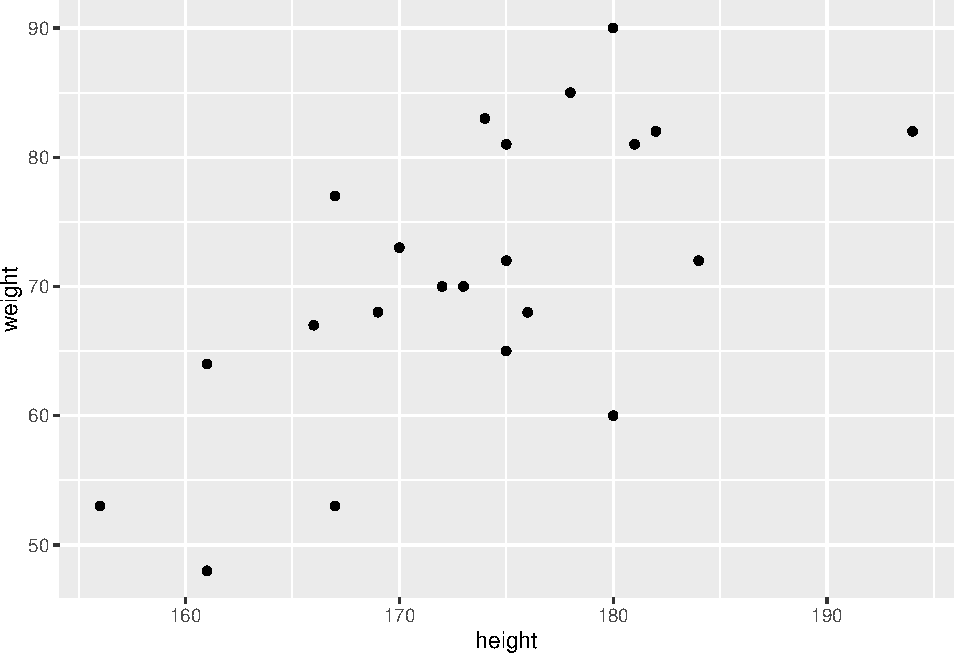
\includegraphics{rmd_reg_files/figure-latex/pressure-1.pdf}

\newpage

\hypertarget{include-a-regression-line}{%
\subsection{Include a regression line:}\label{include-a-regression-line}}

\begin{Shaded}
\begin{Highlighting}[]
\FunctionTok{ggplot}\NormalTok{(classdata, }\FunctionTok{aes}\NormalTok{(}\AttributeTok{x=}\NormalTok{height, }\AttributeTok{y=}\NormalTok{weight)) }\SpecialCharTok{+}
  \FunctionTok{geom\_point}\NormalTok{() }\SpecialCharTok{+}
  \FunctionTok{stat\_smooth}\NormalTok{(}\AttributeTok{formula=}\NormalTok{y}\SpecialCharTok{\textasciitilde{}}\NormalTok{x, }\AttributeTok{method=}\StringTok{"lm"}\NormalTok{, }\AttributeTok{se=}\ConstantTok{FALSE}\NormalTok{, }\AttributeTok{colour=}\StringTok{"red"}\NormalTok{, }\AttributeTok{linetype=}\DecValTok{1}\NormalTok{)}
\end{Highlighting}
\end{Shaded}

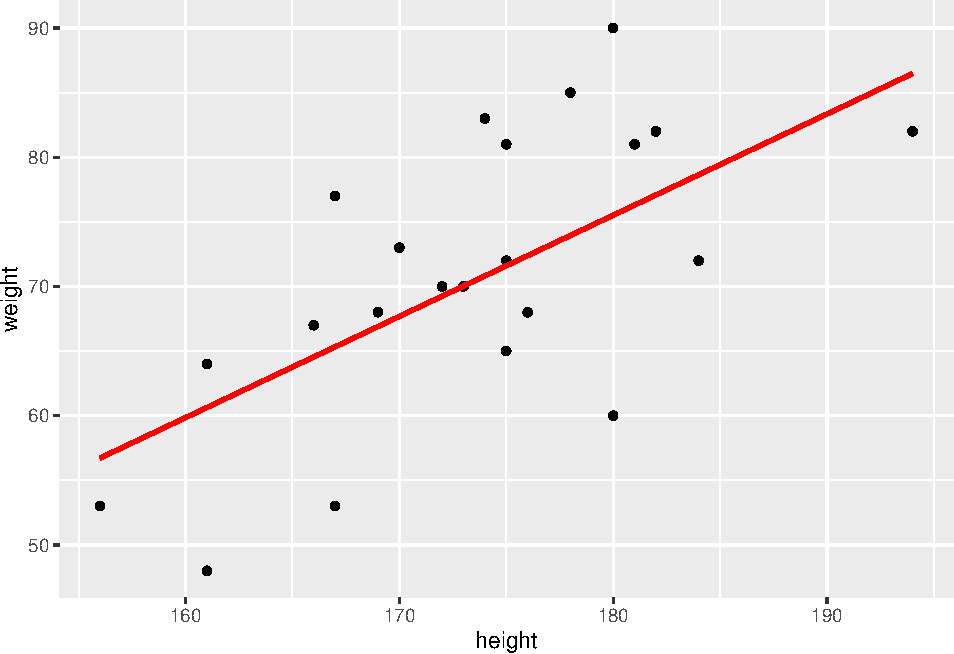
\includegraphics{rmd_reg_files/figure-latex/unnamed-chunk-9-1.pdf}

\newpage

\hypertarget{regression-distinguish-malefemale-by-including-a-seperate-constant}{%
\subsection{Regression: Distinguish male/female by including a seperate constant:}\label{regression-distinguish-malefemale-by-including-a-seperate-constant}}

\begin{Shaded}
\begin{Highlighting}[]
\DocumentationTok{\#\# baseline regression  model}
\NormalTok{model  }\OtherTok{\textless{}{-}} \FunctionTok{lm}\NormalTok{(weight }\SpecialCharTok{\textasciitilde{}}\NormalTok{ height }\SpecialCharTok{+}\NormalTok{ sex , }\AttributeTok{data =}\NormalTok{ classdata )}
\FunctionTok{show}\NormalTok{(model)}
\end{Highlighting}
\end{Shaded}

\begin{verbatim}
## 
## Call:
## lm(formula = weight ~ height + sex, data = classdata)
## 
## Coefficients:
## (Intercept)       height         sexw  
##    -29.5297       0.5923      -5.7894
\end{verbatim}

\begin{Shaded}
\begin{Highlighting}[]
\NormalTok{interm }\OtherTok{\textless{}{-}}\NormalTok{ model}\SpecialCharTok{$}\NormalTok{coefficients[}\DecValTok{1}\NormalTok{] }
\NormalTok{slope  }\OtherTok{\textless{}{-}}\NormalTok{ model}\SpecialCharTok{$}\NormalTok{coefficients[}\DecValTok{2}\NormalTok{]}
\NormalTok{interw }\OtherTok{\textless{}{-}}\NormalTok{ model}\SpecialCharTok{$}\NormalTok{coefficients[}\DecValTok{1}\NormalTok{]}\SpecialCharTok{+}\NormalTok{model}\SpecialCharTok{$}\NormalTok{coefficients[}\DecValTok{3}\NormalTok{] }
\end{Highlighting}
\end{Shaded}

\begin{Shaded}
\begin{Highlighting}[]
\FunctionTok{summary}\NormalTok{(model)}
\end{Highlighting}
\end{Shaded}

\begin{verbatim}
## 
## Call:
## lm(formula = weight ~ height + sex, data = classdata)
## 
## Residuals:
##     Min      1Q  Median      3Q     Max 
## -17.086  -3.730   2.850   7.245  12.914 
## 
## Coefficients:
##             Estimate Std. Error t value Pr(>|t|)  
## (Intercept) -29.5297    47.6606  -0.620   0.5425  
## height        0.5923     0.2671   2.217   0.0383 *
## sexw         -5.7894     4.4773  -1.293   0.2107  
## ---
## Signif. codes:  0 '***' 0.001 '**' 0.01 '*' 0.05 '.' 0.1 ' ' 1
## 
## Residual standard error: 8.942 on 20 degrees of freedom
## Multiple R-squared:  0.4124, Adjusted R-squared:  0.3537 
## F-statistic: 7.019 on 2 and 20 DF,  p-value: 0.004904
\end{verbatim}

\newpage

\begin{Shaded}
\begin{Highlighting}[]
\FunctionTok{ggplot}\NormalTok{(classdata, }\FunctionTok{aes}\NormalTok{(}\AttributeTok{x=}\NormalTok{height, }\AttributeTok{y=}\NormalTok{weight, }\AttributeTok{shape =}\NormalTok{ sex)) }\SpecialCharTok{+}
  \FunctionTok{geom\_point}\NormalTok{() }\SpecialCharTok{+}
  \FunctionTok{geom\_abline}\NormalTok{(}\AttributeTok{slope =}\NormalTok{ slope, }\AttributeTok{intercept =}\NormalTok{ interw, }\AttributeTok{linetype =} \DecValTok{2}\NormalTok{, }\AttributeTok{size=}\FloatTok{1.5}\NormalTok{)}\SpecialCharTok{+}
  \FunctionTok{geom\_abline}\NormalTok{(}\AttributeTok{slope =}\NormalTok{ slope, }\AttributeTok{intercept =}\NormalTok{ interm, }\AttributeTok{linetype =} \DecValTok{2}\NormalTok{, }\AttributeTok{size=}\FloatTok{1.5}\NormalTok{) }\SpecialCharTok{+}
  \FunctionTok{geom\_abline}\NormalTok{(}\AttributeTok{slope =} \FunctionTok{coef}\NormalTok{(model)[[}\DecValTok{2}\NormalTok{]], }\AttributeTok{intercept =} \FunctionTok{coef}\NormalTok{(model)[[}\DecValTok{1}\NormalTok{]]) }
\end{Highlighting}
\end{Shaded}

\begin{verbatim}
## Warning: Using `size` aesthetic for lines was deprecated in ggplot2 3.4.0.
## i Please use `linewidth` instead.
## This warning is displayed once every 8 hours.
## Call `lifecycle::last_lifecycle_warnings()` to see where this warning was generated.
\end{verbatim}

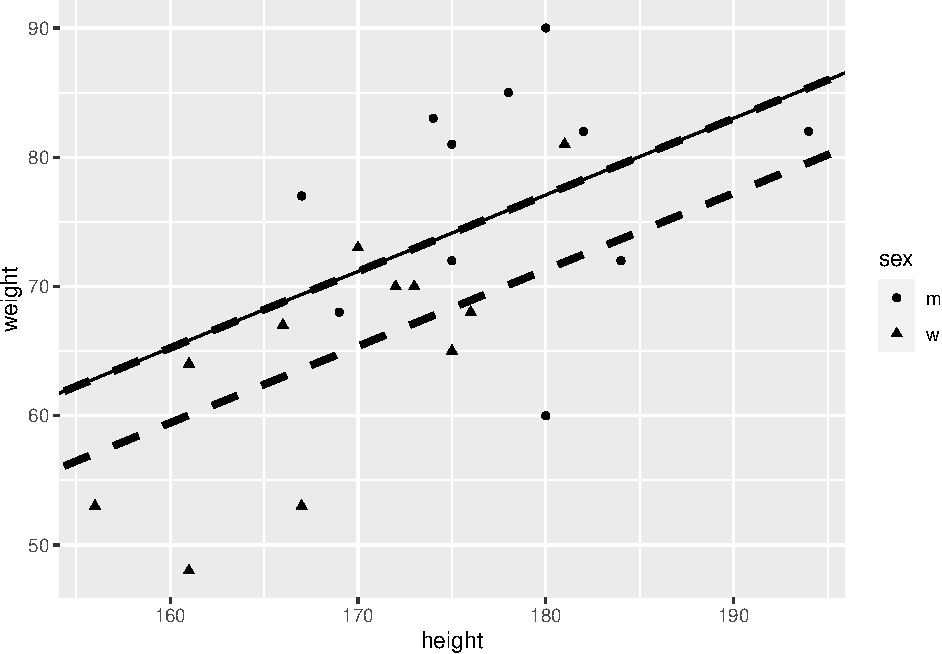
\includegraphics{rmd_reg_files/figure-latex/unnamed-chunk-12-1.pdf}

\newpage

That does not look good. Maybe we should introduce also different slopes for male and female.

\begin{Shaded}
\begin{Highlighting}[]
\FunctionTok{ggplot}\NormalTok{(classdata, }\FunctionTok{aes}\NormalTok{(}\AttributeTok{x=}\NormalTok{height, }\AttributeTok{y=}\NormalTok{weight, }\AttributeTok{shape =}\NormalTok{ sex)) }\SpecialCharTok{+}
  \FunctionTok{geom\_point}\NormalTok{( }\FunctionTok{aes}\NormalTok{(}\AttributeTok{size =} \DecValTok{2}\NormalTok{)) }\SpecialCharTok{+}
  \FunctionTok{stat\_smooth}\NormalTok{(}\AttributeTok{formula =}\NormalTok{ y }\SpecialCharTok{\textasciitilde{}}\NormalTok{ x,  }\AttributeTok{method =} \StringTok{"lm"}\NormalTok{, }
              \AttributeTok{se =} \ConstantTok{FALSE}\NormalTok{, }\AttributeTok{colour =} \StringTok{"red"}\NormalTok{, }\AttributeTok{linetype =} \DecValTok{1}\NormalTok{)}
\end{Highlighting}
\end{Shaded}

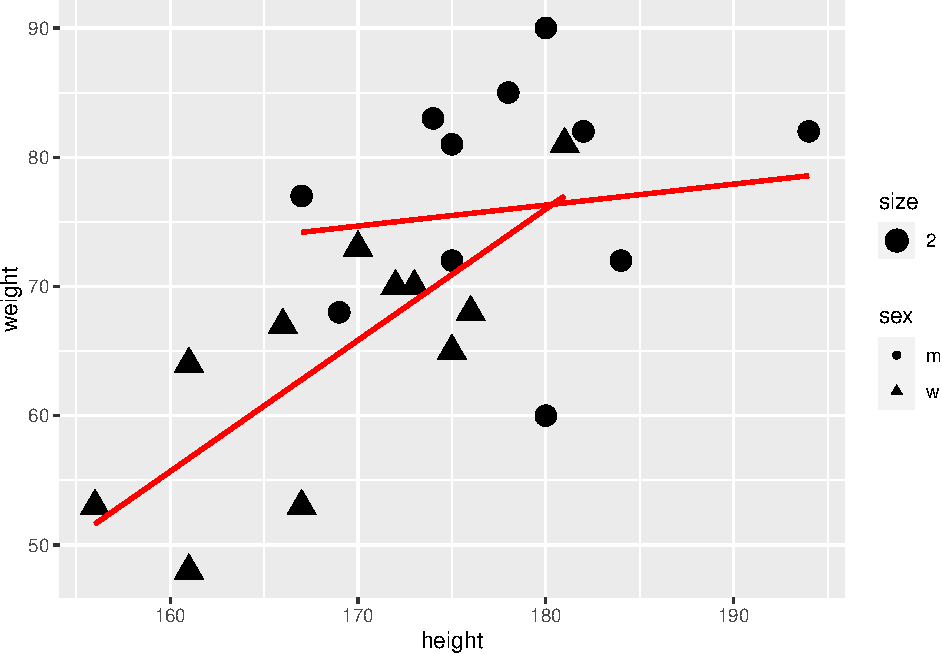
\includegraphics{rmd_reg_files/figure-latex/unnamed-chunk-13-1.pdf}

\newpage

\hypertarget{can-we-use-other-available-variables-such-as-siblings}{%
\subsection{Can we use other available variables such as siblings?}\label{can-we-use-other-available-variables-such-as-siblings}}

\begin{Shaded}
\begin{Highlighting}[]
\FunctionTok{ggplot}\NormalTok{(classdata, }\FunctionTok{aes}\NormalTok{(}\AttributeTok{x=}\NormalTok{height, }\AttributeTok{y=}\NormalTok{weight, }\AttributeTok{shape =}\NormalTok{ sex)) }\SpecialCharTok{+}
  \FunctionTok{geom\_point}\NormalTok{( }\FunctionTok{aes}\NormalTok{(}\AttributeTok{size =}\NormalTok{ siblings)) }
\end{Highlighting}
\end{Shaded}

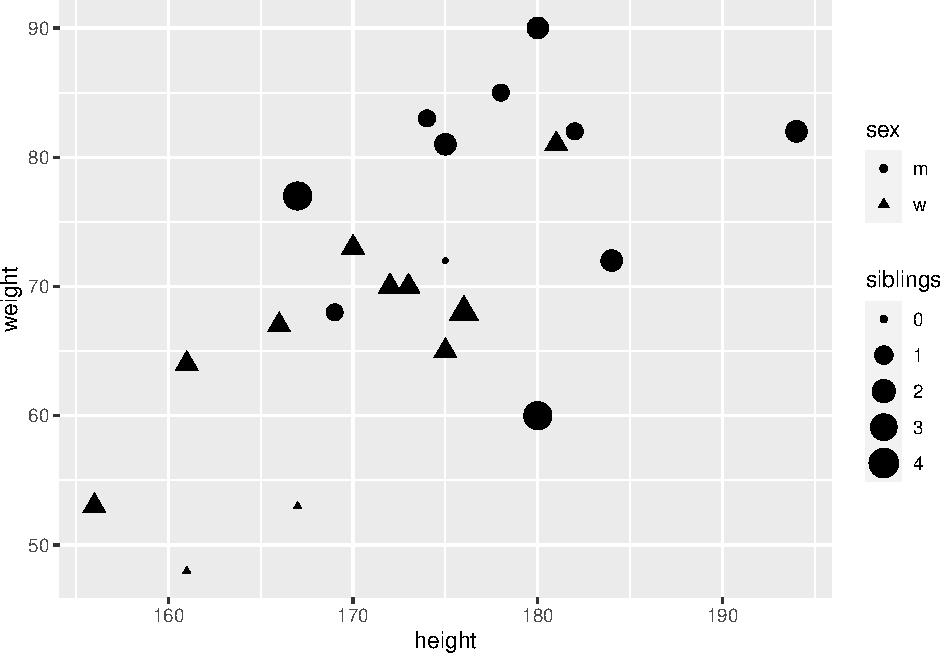
\includegraphics{rmd_reg_files/figure-latex/unnamed-chunk-14-1.pdf}

\begin{Shaded}
\begin{Highlighting}[]
\DocumentationTok{\#\# baseline model}
\NormalTok{model  }\OtherTok{\textless{}{-}} \FunctionTok{lm}\NormalTok{(weight }\SpecialCharTok{\textasciitilde{}}\NormalTok{ height }\SpecialCharTok{+}\NormalTok{ sex , }\AttributeTok{data =}\NormalTok{ classdata )}

\FunctionTok{ggplot}\NormalTok{(classdata, }\FunctionTok{aes}\NormalTok{(}\AttributeTok{x=}\NormalTok{height, }\AttributeTok{y=}\NormalTok{weight, }\AttributeTok{shape =}\NormalTok{ sex)) }\SpecialCharTok{+}
  \FunctionTok{geom\_point}\NormalTok{( }\FunctionTok{aes}\NormalTok{(}\AttributeTok{size =} \DecValTok{2}\NormalTok{)) }\SpecialCharTok{+}
  \FunctionTok{stat\_smooth}\NormalTok{(}\AttributeTok{formula =}\NormalTok{ y }\SpecialCharTok{\textasciitilde{}}\NormalTok{ x,  }
              \AttributeTok{method =} \StringTok{"lm"}\NormalTok{, }
              \AttributeTok{se =}\NormalTok{ T, }
              \AttributeTok{colour =} \StringTok{"red"}\NormalTok{, }
              \AttributeTok{linetype =} \DecValTok{1}\NormalTok{)}
\end{Highlighting}
\end{Shaded}

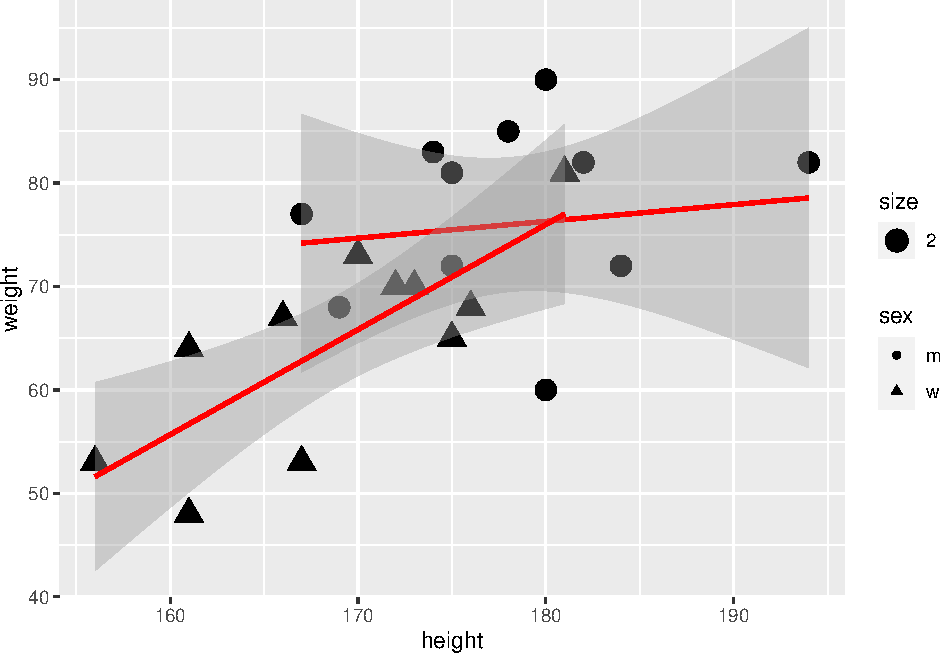
\includegraphics{rmd_reg_files/figure-latex/unnamed-chunk-15-1.pdf}

\newpage

\hypertarget{let-us-look-at-regression-output}{%
\subsection{Let us look at regression output:}\label{let-us-look-at-regression-output}}

\begin{Shaded}
\begin{Highlighting}[]
\NormalTok{m1 }\OtherTok{\textless{}{-}} \FunctionTok{lm}\NormalTok{(weight }\SpecialCharTok{\textasciitilde{}}\NormalTok{ height , }\AttributeTok{data =}\NormalTok{ classdata )}
\NormalTok{m2 }\OtherTok{\textless{}{-}} \FunctionTok{lm}\NormalTok{(weight }\SpecialCharTok{\textasciitilde{}}\NormalTok{ height }\SpecialCharTok{+}\NormalTok{ sex , }\AttributeTok{data =}\NormalTok{ classdata )}
\NormalTok{m3 }\OtherTok{\textless{}{-}} \FunctionTok{lm}\NormalTok{(weight }\SpecialCharTok{\textasciitilde{}}\NormalTok{ height }\SpecialCharTok{+}\NormalTok{ sex }\SpecialCharTok{+}\NormalTok{ height }\SpecialCharTok{*}\NormalTok{ sex , }\AttributeTok{data =}\NormalTok{ classdata )}
\NormalTok{m4 }\OtherTok{\textless{}{-}} \FunctionTok{lm}\NormalTok{(weight }\SpecialCharTok{\textasciitilde{}}\NormalTok{ height }\SpecialCharTok{+}\NormalTok{ sex }\SpecialCharTok{+}\NormalTok{ height }\SpecialCharTok{*}\NormalTok{ sex }\SpecialCharTok{+}\NormalTok{ siblings , }\AttributeTok{data =}\NormalTok{ classdata )}
\NormalTok{m5 }\OtherTok{\textless{}{-}} \FunctionTok{lm}\NormalTok{(weight }\SpecialCharTok{\textasciitilde{}}\NormalTok{ height }\SpecialCharTok{+}\NormalTok{ sex }\SpecialCharTok{+}\NormalTok{ height }\SpecialCharTok{*}\NormalTok{ sex , }\AttributeTok{data =} \FunctionTok{subset}\NormalTok{(classdata, siblings }\SpecialCharTok{\textless{}} \DecValTok{4}\NormalTok{ ))}
\end{Highlighting}
\end{Shaded}

\newpage

\begin{table}[!htbp] \centering 
  \caption{Regression} 
  \label{} 
\small 
\begin{tabular}{@{\extracolsep{5pt}}lccccc} 
\\[-1.8ex]\hline 
\hline \\[-1.8ex] 
 & \multicolumn{5}{c}{\textit{Dependent variable:}} \\ 
\cline{2-6} 
\\[-1.8ex] & \multicolumn{5}{c}{weight} \\ 
 & Model-1 & Model-2 & Model-3 & Model-4 & Model-5 \\ 
\\[-1.8ex] & (1) & (2) & (3) & (4) & (5)\\ 
\hline \\[-1.8ex] 
 height & 0.78$^{***}$ & 0.59$^{**}$ & 0.16 & 0.16 & 0.28 \\ 
  & (0.23) & (0.27) & (0.36) & (0.37) & (0.39) \\ 
  & & & & & \\ 
 sexw &  & $-$5.79 & $-$153.96$^{*}$ & $-$161.92$^{*}$ & $-$134.51 \\ 
  &  & (4.48) & (88.96) & (91.68) & (90.65) \\ 
  & & & & & \\ 
 siblings &  &  &  & $-$1.16 &  \\ 
  &  &  &  & (2.05) &  \\ 
  & & & & & \\ 
 height:sexw &  &  & 0.85 & 0.89 & 0.74 \\ 
  &  &  & (0.51) & (0.53) & (0.52) \\ 
  & & & & & \\ 
 Constant & $-$65.44 & $-$29.53 & 47.14 & 50.27 & 27.69 \\ 
  & (39.35) & (47.66) & (64.81) & (66.23) & (70.36) \\ 
  & & & & & \\ 
\hline \\[-1.8ex] 
Observations & 23 & 23 & 23 & 23 & 21 \\ 
R$^{2}$ & 0.36 & 0.41 & 0.49 & 0.50 & 0.57 \\ 
Adjusted R$^{2}$ & 0.33 & 0.35 & 0.41 & 0.38 & 0.50 \\ 
Residual Std. Error & 9.08 & 8.94 & 8.57 & 8.73 & 8.04 \\ 
F Statistic & 11.98$^{***}$ & 7.02$^{***}$ & 6.02$^{***}$ & 4.44$^{**}$ & 7.59$^{***}$ \\ 
\hline 
\hline \\[-1.8ex] 
\textit{Note:}  & \multicolumn{5}{l}{$^{*}$p$<$0.1; $^{**}$p$<$0.05; $^{***}$p$<$0.01} \\ 
 & \multicolumn{5}{l}{Here are my notes.} \\ 
\end{tabular} 
\end{table}

\newpage

\hypertarget{interpretation-of-the-results}{%
\subsection{Interpretation of the results}\label{interpretation-of-the-results}}

\begin{itemize}
\tightlist
\item
  We can make predictions about the impact of height on male and female
\item
  As both, the intercept and the slope differs for male and female we should interpret the regressions seperately:
\item
  One centimeter more for \textbf{MEN} is \emph{on average} and \emph{ceteris paribus} related with 0.16 kg more weight.
\item
  One centimeter more for \textbf{WOMEN} is \emph{on average} and \emph{ceteris paribus} related with 1.01 kg more weight.
\end{itemize}

\hypertarget{regression-diagnostics}{%
\subsection{Regression Diagnostics}\label{regression-diagnostics}}

Linear Regression makes several assumptions about the data, the model assumes that:

\begin{itemize}
\tightlist
\item
  The relationship between the predictor (x) and the dependent variable (y) has linear relationship.
\item
  The residuals are assumed to have a constant variance.
\item
  The residual errors are assumed to be normally distributed.
\item
  Error terms are independent and have zero mean.
\end{itemize}

More on regression Diagnostics can be found \href{https://daviddalpiaz.github.io/appliedstats/model-diagnostics.html\#r-markdown-6}{Applied Statistics with R: 13 Model Diagnostics}

\newpage

\hypertarget{weighting}{%
\section{Weighting}\label{weighting}}

The formula for the weighted mean is:
\[
\bar{x} = \frac{\sum_{i=1}^{n} w_i \cdot x_i}{\sum_{i=1}^{n} w_i}
\]

In this formula:

\begin{itemize}
\tightlist
\item
  \(\bar{x}\) represents the weighted mean.
\item
  \(n\) is the number of observations.
\item
  \(w_i\) represents the weight for the \(i\)-th observation.
\item
  \(x_i\) represents the \(i\)-th observation value.
\end{itemize}

\begin{Shaded}
\begin{Highlighting}[]
\FunctionTok{rm}\NormalTok{(}\AttributeTok{list =} \FunctionTok{ls}\NormalTok{())}
\NormalTok{wt }\OtherTok{\textless{}{-}} \FunctionTok{c}\NormalTok{(}\DecValTok{5}\NormalTok{, }\DecValTok{2}\NormalTok{, }\DecValTok{2}\NormalTok{, }\DecValTok{1}\NormalTok{)}
\NormalTok{x }\OtherTok{\textless{}{-}} \FunctionTok{c}\NormalTok{(}\DecValTok{1}\NormalTok{, }\DecValTok{2}\NormalTok{, }\DecValTok{3}\NormalTok{, }\DecValTok{4}\NormalTok{)}
\NormalTok{x\_mean }\OtherTok{\textless{}{-}} \FunctionTok{mean}\NormalTok{(x)}
\NormalTok{x\_mean}
\end{Highlighting}
\end{Shaded}

\begin{verbatim}
## [1] 2.5
\end{verbatim}

\begin{Shaded}
\begin{Highlighting}[]
\NormalTok{x\_wt\_mean\_1 }\OtherTok{\textless{}{-}} \FunctionTok{weighted.mean}\NormalTok{(x, wt)}
\NormalTok{x\_wt\_mean\_1}
\end{Highlighting}
\end{Shaded}

\begin{verbatim}
## [1] 1.9
\end{verbatim}

Let us calculate the weighted mean manually:

\begin{Shaded}
\begin{Highlighting}[]
\NormalTok{product }\OtherTok{\textless{}{-}}\NormalTok{ wt}\SpecialCharTok{*}\NormalTok{x}
\CommentTok{\# Nominator}
\NormalTok{nom }\OtherTok{\textless{}{-}} \FunctionTok{sum}\NormalTok{(product)}
\NormalTok{nom}
\end{Highlighting}
\end{Shaded}

\begin{verbatim}
## [1] 19
\end{verbatim}

\begin{Shaded}
\begin{Highlighting}[]
\CommentTok{\# Denominator}
\NormalTok{denom }\OtherTok{\textless{}{-}} \FunctionTok{sum}\NormalTok{(wt)}
\NormalTok{denom}
\end{Highlighting}
\end{Shaded}

\begin{verbatim}
## [1] 10
\end{verbatim}

\begin{Shaded}
\begin{Highlighting}[]
\NormalTok{x\_wt\_mean\_2 }\OtherTok{\textless{}{-}}\NormalTok{ nom}\SpecialCharTok{/}\NormalTok{denom}
\NormalTok{x\_wt\_mean\_2}
\end{Highlighting}
\end{Shaded}

\begin{verbatim}
## [1] 1.9
\end{verbatim}

\newpage

\hypertarget{exercise-1}{%
\subsection{Exercise 1}\label{exercise-1}}

Below you see an alternative way to calculate the weighted mean. Can you explain it?

\begin{Shaded}
\begin{Highlighting}[]
\NormalTok{w\_div\_sumw }\OtherTok{\textless{}{-}}\NormalTok{ wt}\SpecialCharTok{/}\NormalTok{denom}
\NormalTok{w\_div\_sumw}
\end{Highlighting}
\end{Shaded}

\begin{verbatim}
## [1] 0.5 0.2 0.2 0.1
\end{verbatim}

\begin{Shaded}
\begin{Highlighting}[]
\NormalTok{multi\_ww\_x }\OtherTok{\textless{}{-}}\NormalTok{ w\_div\_sumw }\SpecialCharTok{*}\NormalTok{ x}
\NormalTok{multi\_ww\_x}
\end{Highlighting}
\end{Shaded}

\begin{verbatim}
## [1] 0.5 0.4 0.6 0.4
\end{verbatim}

\begin{Shaded}
\begin{Highlighting}[]
\NormalTok{x\_wt\_mean\_3 }\OtherTok{\textless{}{-}} \FunctionTok{sum}\NormalTok{(multi\_ww\_x)}
\NormalTok{x\_wt\_mean\_3}
\end{Highlighting}
\end{Shaded}

\begin{verbatim}
## [1] 1.9
\end{verbatim}

\newpage

\hypertarget{exercise-2}{%
\subsection{Exercise 2}\label{exercise-2}}

\begin{enumerate}
\def\labelenumi{\alph{enumi})}
\tightlist
\item
  Calculate mean, variance, weighted mean, and the variance of the weighted mean for \texttt{x}.
\end{enumerate}

\begin{Shaded}
\begin{Highlighting}[]
\NormalTok{results }\OtherTok{\textless{}{-}} \FunctionTok{data.frame}\NormalTok{(}
  \AttributeTok{Statistic =} \FunctionTok{c}\NormalTok{(}\StringTok{"Mean"}\NormalTok{, }\StringTok{"Variance"}\NormalTok{, }\StringTok{"Weighted Mean"}\NormalTok{, }\StringTok{"Weighted Variance"}\NormalTok{),}
  \AttributeTok{Value =} \FunctionTok{c}\NormalTok{(}\FunctionTok{mean}\NormalTok{(x), }\FunctionTok{var}\NormalTok{(x), }\FunctionTok{weighted.mean}\NormalTok{(x, wt), }\FunctionTok{sum}\NormalTok{(wt }\SpecialCharTok{*}\NormalTok{ (x }\SpecialCharTok{{-}} \FunctionTok{weighted.mean}\NormalTok{(x, wt))}\SpecialCharTok{\^{}}\DecValTok{2}\NormalTok{) }\SpecialCharTok{/} \FunctionTok{sum}\NormalTok{(wt))}
\NormalTok{)}
\FunctionTok{print}\NormalTok{(results)}
\end{Highlighting}
\end{Shaded}

\begin{verbatim}
##           Statistic    Value
## 1              Mean 2.500000
## 2          Variance 1.666667
## 3     Weighted Mean 1.900000
## 4 Weighted Variance 1.090000
\end{verbatim}

\begin{enumerate}
\def\labelenumi{\alph{enumi})}
\setcounter{enumi}{1}
\tightlist
\item
  Do it again but use \texttt{tidyverse} and the function \texttt{summarize}.
\end{enumerate}

\begin{Shaded}
\begin{Highlighting}[]
\NormalTok{df }\OtherTok{\textless{}{-}} \FunctionTok{tibble}\NormalTok{(}\AttributeTok{wt =}\NormalTok{ wt, }\AttributeTok{x =}\NormalTok{ x)}

\NormalTok{summary\_stats }\OtherTok{\textless{}{-}}\NormalTok{ df }\SpecialCharTok{\%\textgreater{}\%}
  \FunctionTok{summarize}\NormalTok{(}
    \AttributeTok{Mean =} \FunctionTok{mean}\NormalTok{(x),}
    \AttributeTok{Variance =} \FunctionTok{var}\NormalTok{(x),}
    \AttributeTok{Weighted\_Mean =} \FunctionTok{weighted.mean}\NormalTok{(x, wt),}
    \AttributeTok{Weighted\_Variance =} \FunctionTok{sum}\NormalTok{(wt }\SpecialCharTok{*}\NormalTok{ (x }\SpecialCharTok{{-}} \FunctionTok{weighted.mean}\NormalTok{(x, wt))}\SpecialCharTok{\^{}}\DecValTok{2}\NormalTok{) }\SpecialCharTok{/} \FunctionTok{sum}\NormalTok{(wt)}
\NormalTok{  )}

\CommentTok{\# Display the table}
\FunctionTok{print}\NormalTok{(summary\_stats)}
\end{Highlighting}
\end{Shaded}

\begin{verbatim}
## # A tibble: 1 x 4
##    Mean Variance Weighted_Mean Weighted_Variance
##   <dbl>    <dbl>         <dbl>             <dbl>
## 1   2.5     1.67           1.9              1.09
\end{verbatim}

\hypertarget{references}{%
\section*{References}\label{references}}
\addcontentsline{toc}{section}{References}

\hypertarget{refs}{}
\begin{CSLReferences}{1}{0}
\leavevmode\vadjust pre{\hypertarget{ref-Wysocki2022Statistical}{}}%
Wysocki, A. C., Lawson, K. M., \& Rhemtulla, M. (2022). Statistical control requires causal justification. \emph{Advances in Methods and Practices in Psychological Science}, \emph{5}(2). \url{https://doi.org/10.1177/25152459221095823}

\end{CSLReferences}


\end{document}
